\chapter{\IfLanguageName{dutch}{Stand van zaken}{State of the art}}%
\label{ch:stand-van-zaken}


% Tip: Begin elk hoofdstuk met een paragraaf inleiding die beschrijft hoe
% dit hoofdstuk past binnen het geheel van de bachelorproef. Geef in het
% bijzonder aan wat de link is met het vorige en volgende hoofdstuk.

% Pas na deze inleidende paragraaf komt de eerste sectiehoofding.
\begin{comment}
Dit hoofdstuk bevat je literatuurstudie. De inhoud gaat verder op de inleiding, maar zal het onderwerp van de bachelorproef *diepgaand* uitspitten. De bedoeling is dat de lezer na lezing van dit hoofdstuk helemaal op de hoogte is van de huidige stand van zaken (state-of-the-art) in het onderzoeksdomein. Iemand die niet vertrouwd is met het onderwerp, weet nu voldoende om de rest van het verhaal te kunnen volgen, zonder dat die er nog andere informatie moet over opzoeken \autocite{Pollefliet2011}.

Je verwijst bij elke bewering die je doet, vakterm die je introduceert, enz.\ naar je bronnen. In \LaTeX{} kan dat met het commando \texttt{$\backslash${textcite\{\}}} of \texttt{$\backslash${autocite\{\}}}. Als argument van het commando geef je de ``sleutel'' van een ``record'' in een bibliografische databank in het Bib\LaTeX{}-formaat (een tekstbestand). Als je expliciet naar de auteur verwijst in de zin (narratieve referentie), gebruik je \texttt{$\backslash${}textcite\{\}}. Soms is de auteursnaam niet expliciet een onderdeel van de zin, dan gebruik je \texttt{$\backslash${}autocite\{\}} (referentie tussen haakjes). Dit gebruik je bv.~bij een citaat, of om in het bijschrift van een overgenomen afbeelding, broncode, tabel, enz. te verwijzen naar de bron. In de volgende paragraaf een voorbeeld van elk.

\textcite{Knuth1998} schreef een van de standaardwerken over sorteer- en zoekalgoritmen. Experten zijn het erover eens dat cloud computing een interessante opportuniteit vormen, zowel voor gebruikers als voor dienstverleners op vlak van informatietechnologie~\autocite{Creeger2009}.

Let er ook op: het \texttt{cite}-commando voor de punt, dus binnen de zin. Je verwijst meteen naar een bron in de eerste zin die erop gebaseerd is, dus niet pas op het einde van een paragraaf.
\end{comment}
(TODO: omzetten markdown naar latex + sources bijzetten + history aanvullen + use case zoeken bij echt bedrijf + opmaak van tussentitels fixen)
\section{SharePoint: Wat Is Het?} 
SharePoint, een multifunctioneel platform ontwikkeld door Microsoft, voorziet samenwerking en informatiebeheer binnen organisaties. Door Sharepoint kan een organisatie al zijn documenten op 1 centrale plek bewaren die door de juiste mensen (met de correcte rechten) gelezen kan worden. Het biedt een brede set aan functies voor documentbeheer, samenwerking, en het bouwen van intranet sites. Het werkt als intranet voor bedrijven waar ze op een veilige manier informatie kunnen delen en  documenten kunnen publiceren binnen het bedrijf of binnen een bepaald project. Sharepoint biedt enkele voordelen zoals beveiligingscontroles, co-authoring, versioning, etc... Al deze tools verbeteren de productiviteit van het bedrijf. \autocite{Willis2024}

\section{Geschiedenis en opkomst} 
SharePoint heeft een interessante reis achter de rug, van zijn eerste lancering tot het worden van de veelgebruikte samenwerkingstool die het nu is. De eerste verschijning van Sharepoint was tijdens de ontwikkelingscyclus van Office XP, dit is de periode waarin Microsoft Office XP ontwikkelde en klaarmaakte voor release in 2001. \autocite{2014} Het doel was sinds het begin al om voor samenwerking te zorgen. De eerste release was een simpele webapplicatie die werknemers toeliet om documenten te delen. In 2003 werd de naam Sharepoint Portal Server en had het al meer functies zoals het opzoeken van documenten. In 2007 kwam Microsoft Office Sharepoint Server 2007 uit en deze had meer features die focsut op de interesses van de bedrijven zelfs. \autocite{Experts2023} De eerste relevante versies waren: SharePoint Foundation 2010, SharePoint Foundation 2013, SharePoint Online, SharePoint Server 2016/SharePoint Enterprise 2016 en SharePoint Server 2019/SharePoint Enterprise 2019. \autocite{Davenport2024} \autocite{Abramenko2016}

\section{Basiscomponenten van SharePoint}

De structuur van elke SharePoint-omgeving is opgebouwd uit verschillende fundamentele componenten die samenwerken om een omgeving voor samenwerking en informatiebeheer aan te bieden. Dit zijn de 3 belangrijkste componenten:
\begin{itemize}
    \item Sites: Sharepoint sites zijn containers met informatie, als je Sharepoint ziet als een universiteit, dan kan je 1 Sharepoint site vergelijken met 1 gebouw binnen de universiteit en zo kun je meerdere gebouwen hebben die deel uitmaken van de hele school. Het gebouw in deze analogie bevat dan informatie. Je kan het ook vergelijken met een smartphone (zie onderstaande figuur) waarbij de Sharepoint site de hele smartphone is. Meestal worden Sharepoint sites per departement aangemaakt omdat dit makkelijker is om beveiligingsregels toe te passen. \autocite{Zelfond2016}
    \item Pagina's: Sharepoint pagina's zijn pagina's die informatie bevatten en dit ook weergeven. Een Sharepoint site kan meerdere Sharepoint pagina's hebben. Er kunnen geen beveiligingsregels worden toegepast op specifieke Sharepoint pagina's zoals dit kan bij sites. Sharepoint pagina's komen overeen met de verschillende schermen waar je tussen kunt scrollen op de startpagina van je smartphone. \autocite{Zelfond2016}
    \item Webonderdelen: Als laatste belangrijke component van Sharepoint zijn er webonderdelen, dit zijn applicaties die zijn geïntegreerd in Sharepoint en voor verschillende doeleinden gebruikt kunnen worden. Webonderdelen komen overeen met de apps op je smartphone. Zo heb je een webonderdeel die documenten opslaat, events opslaat, taken bijhoudt, documenten laat ondertekenen, etc...\autocite{Zelfond2016}
\end{itemize}
\begin{figure}[h] 
    %\centering  This will center the image
    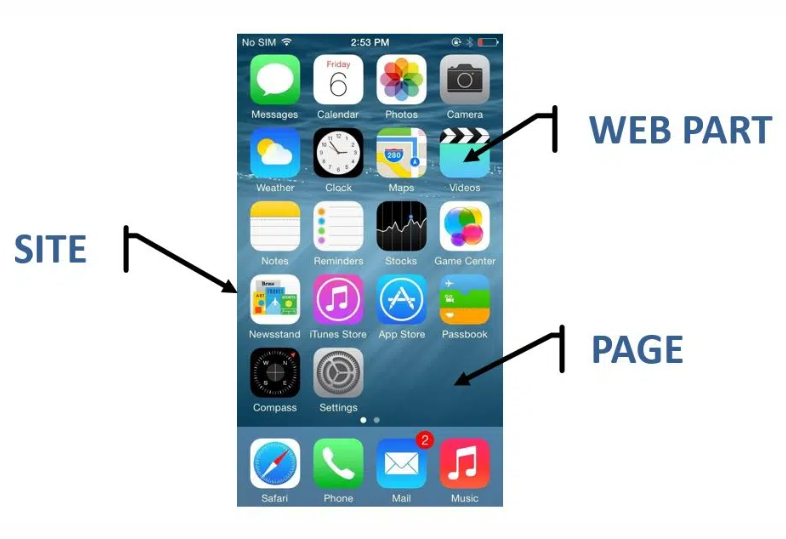
\includegraphics[width=0.5\textwidth]{comps.png} % Adjust the scale or width as needed
    \caption{Visuele voorstelling voor de sites, pagina's en webonderdelen \autocite{Zelfond2016} } % Your caption/subtext goes here
    \label{fig:your_label} % For referencing the figure in your text
\end{figure}

\section{Architectuur}


SharePoint-architectuur vormt de ruggengraat van het platform en is ontworpen om een breed scala aan zakelijke behoeften te ondersteunen, waaronder documentbeheer, samenwerking, het bouwen van bedrijfsprocessen en intranetportalen. Centraal in de architectuur staan webapplicaties, sitecollecties, sites, lijsten en bibliotheken, die gezamenlijk functioneren om content effectief te organiseren en te beheren. Deze componenten stellen organisaties in staat om de structuur en navigatie van het platform aan te passen, waardoor een op maat gemaakte oplossing ontstaat die bijdraagt aan verbeterde efficiëntie en productiviteit. Een belangrijk kenmerk van SharePoint is de modulariteit, voornamelijk geïmplementeerd door webonderdelen en apps. Deze bieden aanpasbare functionaliteiten voor het weergeven, beheren en interactief maken van content, zonder dat gebruikers over uitgebreide programmeerkennis hoeven te beschikken. De architectuur ondersteunt ook een uitgebreide integratie met Microsoft 365, waardoor gebruikers toegang krijgen tot een reeks online diensten en toepassingen, wat de veelzijdigheid en het gebruiksgemak van het platform verder verhoogt. Over de jaren heeft de architectuur van Sharepoint veel verandering gezien, van initiële versies gericht op basisdocumentbeheer tot de huidige cloud-gebaseerde implementaties die naadloos samenwerken met een breed scala aan cloud-diensten. \autocite{Hu2023}
\section{Kernfunctionaliteiten}

SharePoint biedt een breed scala aan functionaliteiten die organisaties ondersteunen in hun dagelijkse operaties, waaronder:
\begin{itemize}
\item Documentbeheer: Met krachtige functies zoals versiebeheer, goedkeuringsstromen, en metadata management, helpt SharePoint organisaties bij het effectief beheren van hun documenten.
\item Samenwerking: SharePoint faciliteert samenwerking binnen teams door middel van gedeelde werkruimtes, integratie met Microsoft Teams, en real-time bewerkingsmogelijkheden voor documenten.
\item Zoeken: Het platform biedt uitgebreide zoekfunctionaliteiten, waardoor gebruikers snel de informatie kunnen vinden die ze nodig hebben.
\item Intranet en extranet sites: Organisaties kunnen SharePoint gebruiken om intranet sites voor interne communicatie en samenwerking te bouwen, evenals extranet sites voor interactie met externe partijen.
\item Aanpassing en uitbreidbaarheid: SharePoint stelt organisaties in staat om het platform aan te passen en uit te breiden met aangepaste oplossingen en integraties, dankzij een rijke set aan ontwikkelingstools en API's.
\end{itemize}
SharePoint speelt een cruciale rol in het digitale werkpleklandschap van veel organisaties, dankzij de flexibiliteit, schaalbaarheid, en rijke functionaliteit. Door de fundamenten van SharePoint te begrijpen, kunnen organisaties beter bepalen hoe ze het platform effectief kunnen inzetten om hun samenwerkings- en informatiebeheerdoelstellingen te bereiken.



\section{Implementatiemethoden}%
SharePoint, het robuuste platform van Microsoft voor samenwerking en contentbeheer, biedt verschillende implementatiemodellen om tegemoet te komen aan de diverse behoeften van organisaties. Elk implementatiemodel biedt unieke voordelen en aandachtspunten, waardoor het cruciaal is voor bedrijven om het model te kiezen dat het beste aansluit bij hun operationele vereisten, technische capaciteiten en strategische doelen. In deze tekst verkennen we de verschillende implementatiemodellen voor SharePoint: SharePoint Online, SharePoint Server (on-premises) en SharePoint Hybrid.

\subsection{SharePoint Online}
SharePoint Online, een cloudgebaseerde service gehost door Microsoft, maakt deel uit van het Office 365-pakket. Dit model elimineert de noodzaak voor organisaties om de infrastructuur te beheren, aangezien Microsoft zorgt voor de servers, opslag en beveiliging. Dit biedt organisaties het voordeel van schaalbaarheid, waardoor ze gemakkelijk gebruikers kunnen toevoegen of verwijderen en opslagruimte kunnen aanpassen op basis van hun behoeften. Bovendien zorgt SharePoint Online voor automatische updates en patches, wat betekent dat organisaties altijd toegang hebben tot de nieuwste functies en beveiligingsverbeteringen zonder zelf het onderhoud te hoeven beheren. Een belangrijk voordeel is ook de integratie met andere Office 365-diensten, waardoor een naadloze samenwerkingsomgeving ontstaat.

\subsection{SharePoint Server (on-premises)}
Voor organisaties die volledige controle willen behouden over hun SharePoint-omgeving, biedt SharePoint Server een on-premises oplossing. Dit model vereist dat organisaties hun eigen servers, opslag en netwerk beheren. Hoewel dit meer controle en aanpassingsmogelijkheden biedt, brengt het ook de verantwoordelijkheid met zich mee voor het uitvoeren van updates, patches en het beheren van de beveiliging. SharePoint Server is ideaal voor organisaties met strenge gegevensbeveiligingsvereisten of die specifieke aanpassingen en integraties nodig hebben die niet beschikbaar zijn in de cloud. Dit model kan echter hogere initiële en lopende kosten met zich meebrengen vanwege de vereiste voor hardware, softwarelicenties en IT-personeel voor onderhoud.

\subsection{SharePoint Hybrid}
Het hybride model combineert elementen van zowel SharePoint Online als SharePoint Server, waardoor organisaties het beste van twee werelden kunnen benutten. In een hybride omgeving kunnen organisaties sommige gegevens en applicaties in de cloud hosten terwijl ze andere lokaal houden. Dit is bijzonder nuttig voor organisaties die geleidelijk naar de cloud willen migreren of die bepaalde gegevens om regelgevende of beleidsredenen on-premises moeten houden. Een hybride implementatie biedt flexibiliteit in hoe en waar werk wordt gedaan, met naadloze integratie tussen cloud- en on-premises omgevingen, waardoor gebruikers een uniforme ervaring krijgen, ongeacht waar de gegevens worden gehost.

Elk van deze implementatiemodellen heeft zijn eigen set voordelen en uitdagingen, en de keuze voor een specifiek model hangt af van de specifieke behoeften en omstandigheden van een organisatie. Het is belangrijk voor organisaties om hun bedrijfsdoelstellingen, technische vereisten en budgettaire overwegingen zorgvuldig af te wegen bij het kiezen van het meest geschikte SharePoint-implementatiemodel.













